% outline

% title-me
% EBCWA problem
% ideal solution (solution attributes)
% DITA (verse fail http://media.boreme.com/post_media/2008/tank-toll.jpg)
% docutils (nearly success)
%  MS-Word -> docbookXML -> reST
%  recognise verses (1saiah)
%  verse role
%  biblepassage directive
%  document linking/sharing
%  draft-comment
% sphinx
%  conf.py
%  toctree
%  4 types (all html, 1 pdf, 1 epub, 1 google-docs) (bible-version, draft)
% paver
%  paver <type> book <version> <draft> <force>
%  override conf.py with cog
%  run pdflatex with rubber
%  singlehtml->insert css with cog->google-doc

\newcommand{\rst}{reStructuredText}
\documentclass{beamer}
\usepackage{minted}
\usetheme{default}
\hypersetup{colorlinks=true}
\usepackage{framed}
\usepackage[normalem]{ulem}

\title{TheoreST: Publishing Theology with Python}
\subtitle{Kiwi PyCon 2013}
\author{Carl Cerecke}
\institute{Evangelical Bible College of Western Australia}
\date{September 8, 2013}

\begin{document}

    \begin{frame}[plain]
        \titlepage
    \end{frame}

\begin{frame}{Overview of the talk}
    \begin{itemize}
    \item Publishing problem (and ideal solution)
    \item A tank is not the solution
    \item Proprietary format $\rightarrow$ \rst
    \item Domain-specific problems (bible verses)
    \item \rst\ $\rightarrow$ web/pdf/epub (sphinx)
    \item Automating with \texttt{paver} and \texttt{cog}
    \item Todo\ldots
    \end{itemize}
\end{frame}
    
\begin{frame}{The problem}
    \begin{itemize}
    \item $\simeq$300 books in MS Word format (written over 20+ years)
        \begin{itemize}
        \item Systematic Theology
        \item Pastoral Theology
        \item Commentaries
        \item Miscellaneous topics 
        \end{itemize}
    \item Two primary authors. Non-technical
    \item Domain-specific behaviour (verse references)
    \item Distribute as widely and conveniently as possible
    \item ``Freely you have received, freely give''
    \end{itemize}
\end{frame}
    
\begin{frame}{The (ideal) solution}
\begin{itemize}
    \item One authoritative source, multiple outputs
    \item Share common document fragments
    \item Bible version independent
    \item Bible references hyperlinked: \href{http://some.url}{John 3:16}
    \item Build individual books (pdf/epub), or whole collection (html)
    \item Simple method for authors to make changes
\end{itemize}
\end{frame}

    
\begin{frame}{DITA: The Wrong Way}
    \begin{itemize}
    \item DITA: Darwin Information Typing Architecture
    \item \url{http://dita.xml.org/}
    \item `Enterprise-level' technical documentation
    \item XML
    \item Java
    \item Complex
    \item Deal-breaker: Too static\ldots\\
        Dynamically determine bible-reference URLs during document creation? Too hard.
    \end{itemize}
\end{frame}

\begin{frame}[plain]
    \centerline{
\includegraphics[keepaspectratio=true, width=\paperwidth]{tank-toll.jpg}}
\end{frame}

\begin{frame}{\rst\ and sphinx: A Better Way}
\begin{itemize}
\item Markup language
\item \url{http://docutils.sourceforge.net/rst.html}
\item Part of docutils text processing system
\item Relatively easy to extend
\item Multiple output formats: html, pdf (via \LaTeX), epub
\item Used by sphinx \url{http://sphinx-doc.org/}
\begin{itemize}
\item Used to generate \url{http://docs.python.org}
\item Extensions for hierarchichal documents
\item Python
\item Not XML!
\end{itemize}
\end{itemize}
\end{frame}


\begin{frame}{\rst\ markup language (PEP 287)}
\centerline{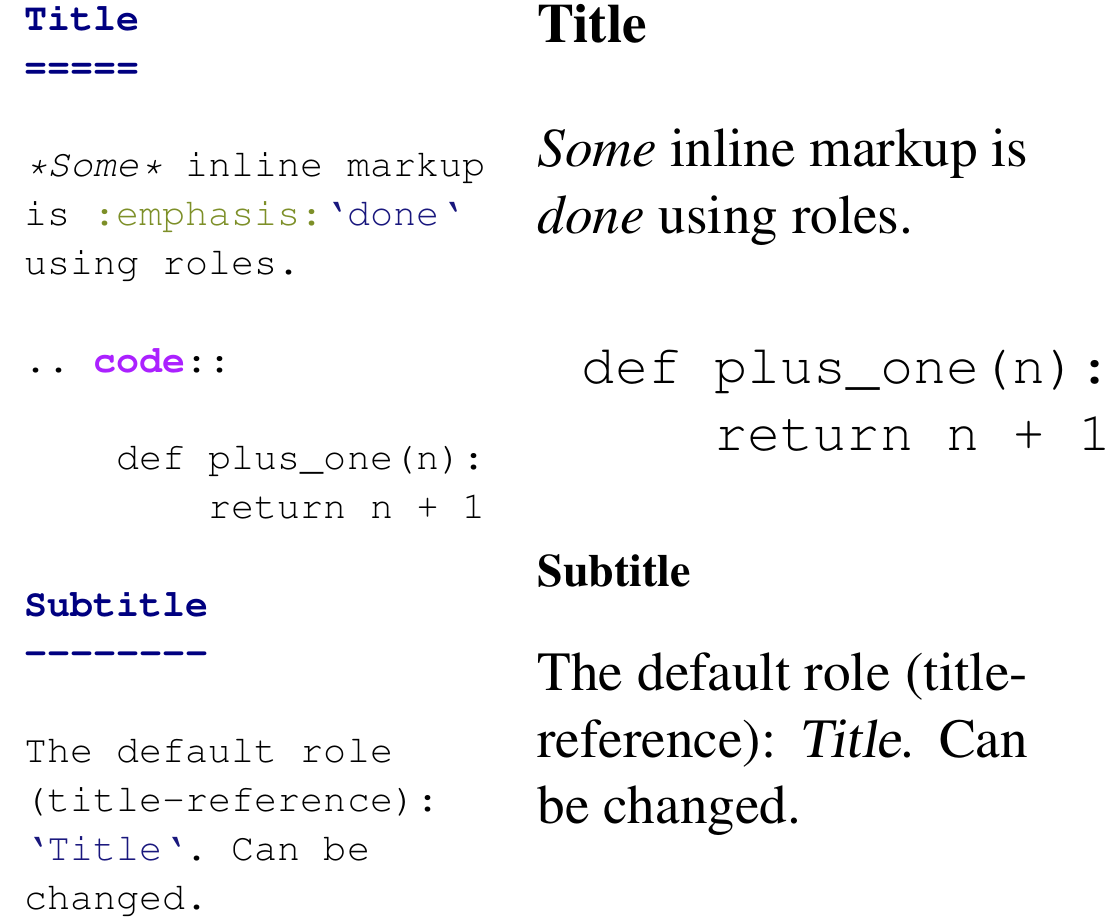
\includegraphics[keepaspectratio=true, width=\paperwidth, height=0.9\paperheight]{rst_example.png}}
\end{frame}

\begin{frame}
    \centerline{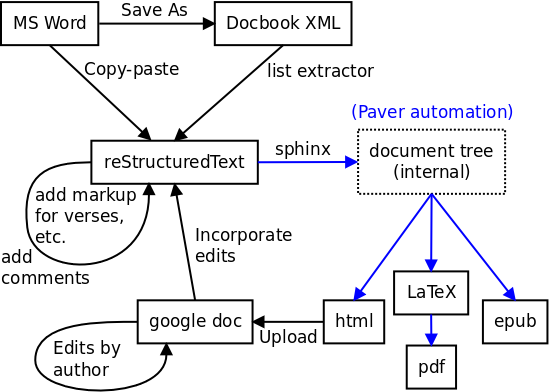
\includegraphics[keepaspectratio=true, width=\paperwidth]{theorest_process.png}}
\end{frame}


\begin{frame}[fragile]{TheoreST technology overview}
\begin{itemize}
\item \url{https://github.com/cdjc/theoreST}
\item python 3.3
\item sphinx
\item paver (build tool)
\item cog (code generation tool)
\item \LaTeX\  and rubber (generating pdf)
\item Linux Mint 15 virtualbox VM
\item Wing IDE Professional (thanks nz pycon!)
\item Google drive/docs
\end{itemize}
\end{frame}

\begin{frame}{MS Word problems}
No styles! What you see is \emph{all} you've got

    \begin{framed} %{enumerated lists}
        \ldots\\
3. PAUL'S TRIALS\\
\quad (a) Persecuted in Damascus; escapes in basket (Acts 9:20-25)\\
\quad (b) Driven out of Jerusalem, sent to Tarsus (Acts 9:28-30)\\
\quad (c) Stoned at Lystra and thought to have died (Acts 14:19)\\
\quad (d) Whipped and imprisoned at Phillipi (Acts 16:16-24)\\
\ldots
\end{framed}
Solution:\\
\emph{Save As...} docbook XML format. Guess indent level
\end{frame}

\begin{frame}[fragile]
    \frametitle{Recognising bible references}
     Want to replace:\\
     \begin{verbatim}Lorem ipsum John 3:16 dolor
\end{verbatim}
     with:\\
 \begin{verbatim}Lorem ipsum `John 3:16` dolor
\end{verbatim}
Other examples:
\begin{itemize}
\item multiple verses: John 3:16,20
\item verse range: John 3:16-20
\item whole chapter: John 3
\item Multi chapter: John 3:16, 4:4
\item Multi book, chapter, verse, range:\\
    John 3:16-18,20,4:1, 3 John 1:2, Luke 1:1
\end{itemize}
\end{frame}

\begin{frame}{Regular expressions}
    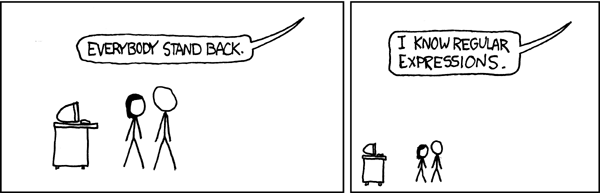
\includegraphics[keepaspectratio=true, width=0.9\paperwidth]{regular_expressions.png}

High-level view of regular expressions:
\begin{itemize}
\item A mini-language for specifying a set of strings
\item An efficient \emph{recogniser} for that set of strings
\end{itemize}

\end{frame}



\begin{frame}[fragile]{Quoting bible references}
    
\begin{minted}{python}
names = ['Genesis', 'Exodus', ..., 'Revelation']
re_names = '('+'|'.join(names)+')'
re_raw = '('+re_names+r'\s+\d+:(\s*(,|-|;|:|'+\
    re_names+'|\d+))+'+')'
re_bibref = re.compile(re_raw)

def bibquote(text):
    return re_bibref.sub(r'`\1`', text)
\end{minted}

\vspace{1cm}

What about lsaiah? or I Corinthians? Argh!

\end{frame}

\begin{frame}%{MS Word format to \rst}
    \centerline{
\includegraphics[keepaspectratio=true, width=\paperwidth]{typewriter_keyboard.jpg}}
\end{frame}

\begin{frame}[fragile]{Parsing the verse roles}
\begin{itemize}
\item Need to translate \texttt{`John 3:16-18,20`} into:

\begin{minted}{html}
<a href="http://bible.xyz/ESV/john3+3:16-18">
John 3:16-18</a>,
<a href="http://bible.xyz/ESV/john3+3:20">20</a>
\end{minted}

\item Actually, internal document-tree nodes representing links
\end{itemize}

\begin{enumerate}
\item Tokenise
\item Parse
\item Output
\end{enumerate}
\end{frame}

\begin{frame}[fragile]{Tokenisation}
Use python's own tokeniser

\begin{minted}{bash}
> echo "John 3:16-18,20" | python3 -m tokenize
1,0-1,4:            NAME           'John'         
1,5-1,6:            NUMBER         '3'            
1,6-1,7:            OP             ':'            
1,7-1,9:            NUMBER         '16'           
1,9-1,10:           OP             '-'            
1,10-1,12:          NUMBER         '18'           
1,12-1,13:          OP             ','            
1,13-1,15:          NUMBER         '20'           
1,15-1,16:          NEWLINE        '\n'           
2,0-2,0:            ENDMARKER      ''             
\end{minted}

\end{frame}

\begin{frame}[fragile]{Parsing}

\begin{itemize}
\item Plenty of parser-generators available
\begin{itemize}
\item \url{http://wiki.python.org/moin/LanguageParsing}

\item But, too heavyweight
\end{itemize}

\item Verse references don't nest

\item But do need lookahead:
\begin{minted}{python}
'John' '3' ':' '16' '-' '18' ',' '20' ...
\end{minted}

\item Solution: Use a state machine!

\pause
\item Problem: No goto :-(

\pause
\item Solution: My goto function decorator:\\
\url{http://code.activestate.com/recipes/576944-the-goto-decorator/}

\pause
\item Problem: Only python 2
\end{itemize}
\end{frame}

\begin{frame}{Avoiding the raptors}
    \centerline{
\includegraphics[keepaspectratio=true, width=\paperwidth]{goto.png}}
\end{frame}


\begin{frame}[fragile]{Parsing state machine (no \texttt{goto}s)}

One method per state

Each method-state returns next method-state

\begin{minted}{python}
def parse(self):
    ...
    state = self.p_book            # start state
    while state:
        state = state()            # 'do' state. get next
		
def p_book(self):                  # expect to parse book
    self.book = self.swallow(Book) # eat Book token
    self.text += self.book.value   # collect link text
    return self.p_chapter          # 'goto' this state
	
def p_chapter(self):               # expecting a chapter
    ...
\end{minted}
\end{frame}

\begin{frame}{Extending \rst/sphinx}

\begin{itemize}
\item Roles (inline markup--- \texttt{:gk:`agape`})
\begin{itemize}
\item Single function; returns doctree nodes
\item \texttt{verse} role (parse verse text, insert references)
\item \texttt{greek} role (nothing much, yet)
\end{itemize}
\item Directives (block markup)
\begin{itemize}
\item Single class with \texttt{run} method. Returns doctree nodes
\item \texttt{biblepassage} directive (inserts bible text into document)
\item \texttt{draftcomment} directive
\end{itemize}
\item Domain (collection of extensions)
\begin{itemize}
\item Roles
\item Directives
\item Config values
\end{itemize}
\end{itemize}

\end{frame}

\begin{frame}{Automating the build process}
\begin{itemize}
\item Problem: minimise effort to build documentation

\item What I want to build:
\begin{itemize}
\item All documents in integrated sphinx website
\item Individual documents as pdf/epub/html-for-google-docs
\end{itemize}
\item For each build I want to specify:
\begin{itemize}
\item bible version (ESV, KJV, NET, etc.)
\item include draft comments
\item possibly other options (e.g. a4/letter)
\end{itemize}
\item Also, minimal duplication in sphinx \texttt{conf.py}\\

\item Solution: paver
\end{itemize}
\end{frame}

\begin{frame}{Automating the build process with paver}

\url{http://paver.github.io/paver/}

\begin{quote}
Paver is a Python-based build/distribution/deployment 
scripting tool along the lines of Make.
\end{quote}

Command line I want:
\begin{itemize}
\item \texttt{paver html} (integrated website with all books)
\item \texttt{paver pdf john} (pdf ouput of John, default bible version)
\item \texttt{paver epub john}
\item \texttt{paver pdf john NET letter} (use NET bible, letter paper)
\item \texttt{paver single john} (html for upload to google-docs)
\item \texttt{paver pdf matthew mark luke john} (multiple books)
\end{itemize}

Sets up configuration, then calls \texttt{sphinx-build}

\end{frame}

\begin{frame}[fragile]{Sharing a single sphinx config file}

\begin{itemize}
\item \texttt{index.rst} is the root of a document
\item \texttt{conf.py} is the sphinx config file
\end{itemize}

Project file hierarchy:

\begin{tabular}{|l|l|}
\hline
\texttt{/} & root directory \\
\hline
\texttt{/index.rst} & Integrated website with all books \\
\texttt{/conf.py} & Symbolic link to \texttt{src/conf.py}\\
\texttt{/conf\_override.py} & Append to \texttt{conf.py}\\
\hline
\texttt{/src/} & Common configuration and code\\
\texttt{/src/conf.py} & Common sphinx configuration file\\
\hline
\texttt{/\emph{group}/\emph{book}/index.rst} & For stand-alone documents\\
\texttt{/\emph{group}/\emph{book}/conf.py} & Symbolic link to \texttt{/src/conf.py}\\
\texttt{/\emph{group}/\emph{book}/conf\_override.py} & Append to \texttt{conf.py}\\
\hline
\end{tabular}


\end{frame}

\begin{frame}[fragile]{Handling sphinx options?}

\begin{itemize}
\item Sphinx configuration file is python code.

\item Can override simple \texttt{name=value} options on command line:\\
\texttt{sphinx-build -Dbible\_version=ESV}

\item But complex overrides (i.e. python code) fail:
\sout{\texttt{-Dlatex\_elements['papersize']='a4paper'}}

\item Some overrides are static per-book:\\
Generated \LaTeX\ filename = \texttt{john.tex}

\item Others are dynamic--- at generation time:
\texttt{papersize = "letter"}
\end{itemize}

Solution: code generation with \emph{cog}
\end{frame}

\begin{frame}[fragile]{Taming the sphinx config file with \emph{cog}}

\url{http://nedbatchelder.com/code/cog/}

\begin{itemize}
\item Cog: Use python code in a file to generate part of that file

\item At the end of sphinx config file:
\begin{minted}{python}
#[[[cog 
#include('conf_override.py')
#cog.out('\n')
#if 'override_text' in globals():
#    cog.out(override_text)
#]]]
#[[[end]]]
\end{minted}

\item Cog runs python code between \texttt{[[[cog} and \texttt{]]]}

\item Output (via \texttt{cog.out}) appears between \texttt{]]]} and \texttt{[[[end]]]}

\item In paver stdlib: \texttt{paver.doctools.cog(\emph{options})}
\end{itemize}
\end{frame}

\begin{frame}[fragile]{The draft-comment-edit cycle}
%\begin{enumerate}
%\item Document in draft form.
%\item Comments are made on that draft
%\item Changes are made based on comments.
%\end{enumerate}

From one of the authors:

\begin{quote}
I come from a pre computer background which means I can write material and
send out emails plus do some limited scanning but nothing else.
\end{quote}

%Editing \rst\ source? I don't think so.

Current Solution:

\begin{enumerate}
\item Publish to html (paver)
\item Upload to google-drive, converting to google doc
\item Author edits google doc
\item I incorporate changes to \rst\ source 
\item If not finished, goto step 1
\end{enumerate}

%Conversion is poor. Need way to programmatically create google docs.

%other options: Wiki, github interface\ldots
\end{frame}


\begin{frame}{Future work}
\begin{itemize}
\item Continue converting documents to reST
\item Robust versioning scheme
\item Translation (with the aid of google-translate)
\item Dynamic bible-version selection on website
\item Greek/Hebrew/Aramaic hyperlinks
\item Website hosting
\item Formatting tweaks
\item Fix bugs. Add more tests
\item Use more github features
\end{itemize}

\end{frame}
\end{document}
